\subsection{An\'alise dos Modelos}

A Figura \ref{fig:1-ar} tem como objetivo apresentar uma previsão de um passo à frente (um dia). Nos apêndices \ref{sec:ararxma24}, pode-se observar uma comparação entre os modelos AR, MA e ARX.
O modelo MA, quando comparado com o modelo AR de mesma ordem, facilita a previsão. Conforme na Figura \ref{fig:1-ma}, a previsão gráfica se assemelha ao modelo apresentado na Figura \ref{fig:1-ar}, embora não seja comparável ao modelo exibido na Figura \ref{fig:1-arx}. É importante notar que esse modelo aparenta prever com precisão o período de tempo que foi considerado.

A Figura \ref{fig:1-arma} combina dos modelos AR e MA em um modelo ARMA. Essa abordagem pode levar a uma redução significativa no erro de previsão, como observado nos apêndices \ref{sec:comtb24} e \ref{sec:comtb18}, onde são apresentadas comparações com um maior número de passos de previsão.
Ao analisar a Figura \ref{fig:1-arima}, não se nota uma diferença visual significativa em relação aos outros métodos apresentados anteriormente. O método ARX ainda parece ser superior aos demais com base na análise visual.

Na Figura \ref{fig:1-sarima}, é possível observar que a previsão em vermelho está mais próxima dos valores observados em preto, mostrando que a inclusão do componente de sazonalidade melhora a qualidade da previsão. Os modelos SARIMA são capazes de lidar com dados que apresentam padrões sazonais, permitindo a diferenciação dos dados em termos de componentes sazonais e não sazonais. Uma abordagem útil para determinar os melhores parâmetros do modelo é utilizar uma estrutura de pesquisa automatizada de parâmetros, como o pmdarima, que auxilia na identificação dos parâmetros ideais para o modelo SARIMA. Isso pode contribuir para uma melhor compreensão e ajuste do modelo aos dados observados.

Entre os modelos com variáveis exógenas, como mostrado nas Figuras \ref{fig:1-arimax} e \ref{fig:1-sarimax}, observa-se uma melhora significativa na qualidade das previsões em comparação com os modelos que não incluem variáveis exógenas. A adição dessas variáveis externas permite capturar melhor as influências e os padrões presentes nos dados, resultando em previsões mais completas e precisas. Essa inclusão de informações adicionais contribui para uma compreensão mais abrangente do comportamento da série temporal e possibilita uma melhor adaptação do modelo aos padrões observados.

Na Figura \ref{fig:prophet1}, é apresentada a previsão da variável LT01 usando o Prophet. Este modelo exibe diversas informações, como a sazonalidade dos dados e a tendência. O Prophet é considerado um modelo mais fácil de ser utilizado em comparação com modelos mais antigos, como o ARIMA. Isso ocorre porque o Prophet é um modelo mais moderno e foi projetado para simplificar o processo de previsão, tornando-o mais acessível para usuários que não possuam conhecimentos avançados em séries temporais. O Prophet é uma escolha atraente para análise e previsão de dados sazonais e tendências.

A Figura \ref{fig:lr-lt01-m3} fornece uma representação visual da interpretação dos coeficientes $\beta_0$ e $\beta_1$. Um aumento de $1$ na variável $x$ está associado a um aumento proporcional de $\beta_1$ na variável $y$. O valor de $\beta_0$ representa o valor de $y$ quando $x$ é igual a $0$.
A Figura \ref{fig:1-regressao-linear}, um passo à frente dos dados da SANEPAR foi previsto. Esse modelo mais simples do que os outros modelos pode ser útil em horizonte menor, mas em horizontes de vários dias ele peca muito. Ele é um dos modelos que mais apresenta erro na análise dos erros sMAPE, MAE e RRMSE.
A Figura \ref{fig:decision-tree-regressor}, é apresentado este modelo com o intuito de corrigir o erro que o LR estava tendo em prever muitos dias à frente. Este modelo, por ser mais robusto, consegue trabalhar na otimização dos hiperparâmetros, tornando-o melhor que o LR na questão de horizontes mais longos.
Na Figura \ref{fig:1-regressao-rfa}, o modelo é construído e analisado em comparação com os outros modelos, e ele se destaca em relação aos modelos anteriores já analisados em um passo à frente.

Na Figura \ref{fig:1-xgb-regressao}, são apresentados os modelos XGBoost e LightGBM. Esses modelos, devido à sua semelhança, exibem tempos de desempenho muito próximos um do outro. Na Figura \ref{fig:xgb}, é exibida uma previsão de um passo à frente, e observa-se que esse modelo parece ser superior aos demais modelos previamente apresentados. Por outro lado, na Figura \ref{fig:lgb}, apesar de ser um modelo mais leve em termos de tempo de computação, ele ainda não atingiu o desempenho esperado para o tema abordado.

Os modelos de rede neural, como RNN, ANN, CNN, GRU, LSTM e Transformer, não foram apresentados aqui, pois não demonstraram tanta relevância no gráfico, mas estão detalhados na tabulação. O modelo RNN é mostrado no Apêndice \ref{sec:arimaxsarimasarimax24}, onde uma comparação com os horizontes de previsão escolhidos é apresentada na Figura \ref{fig:rnn}, exibindo o próprio modelo em si.

\begin{figure}[H]
	\centering
	\caption{Comparação dos modelos AR e ARX}
	\begin{subfigure}{1\textwidth}
			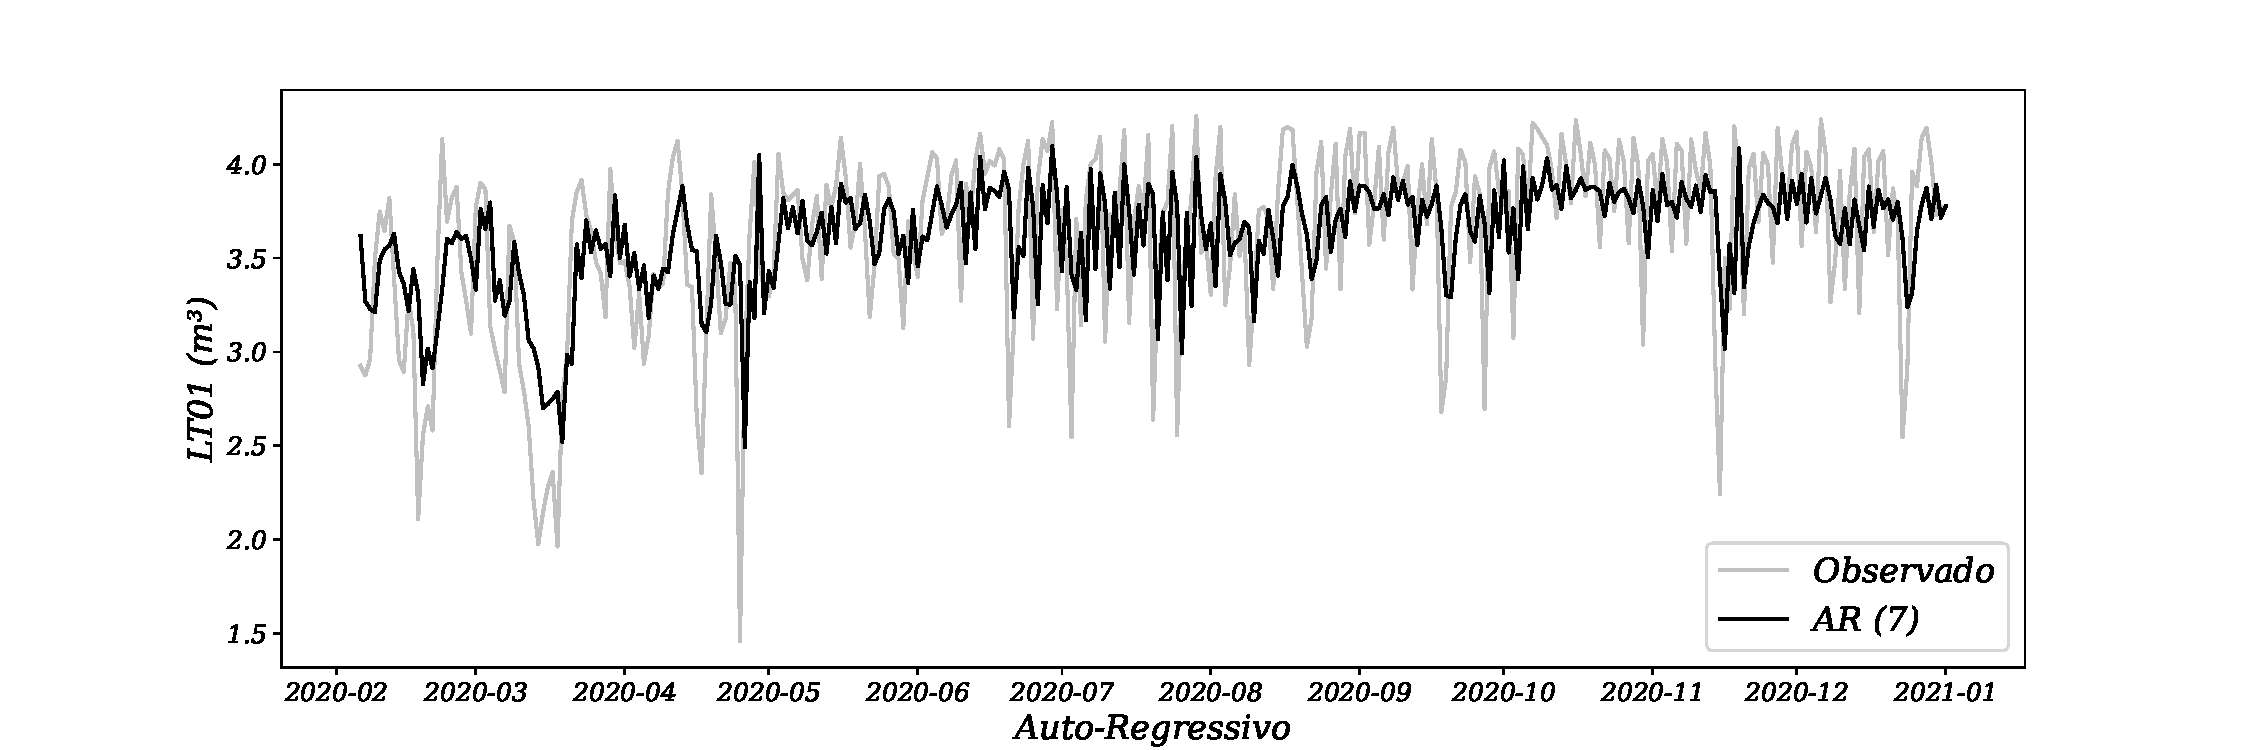
\includegraphics[width=\linewidth]{Modelos/Figuras/AR}
			\caption{Modelo AR(7)}
			\label{fig:1-ar}	
		\end{subfigure}
	
	\begin{subfigure}{1\textwidth}
			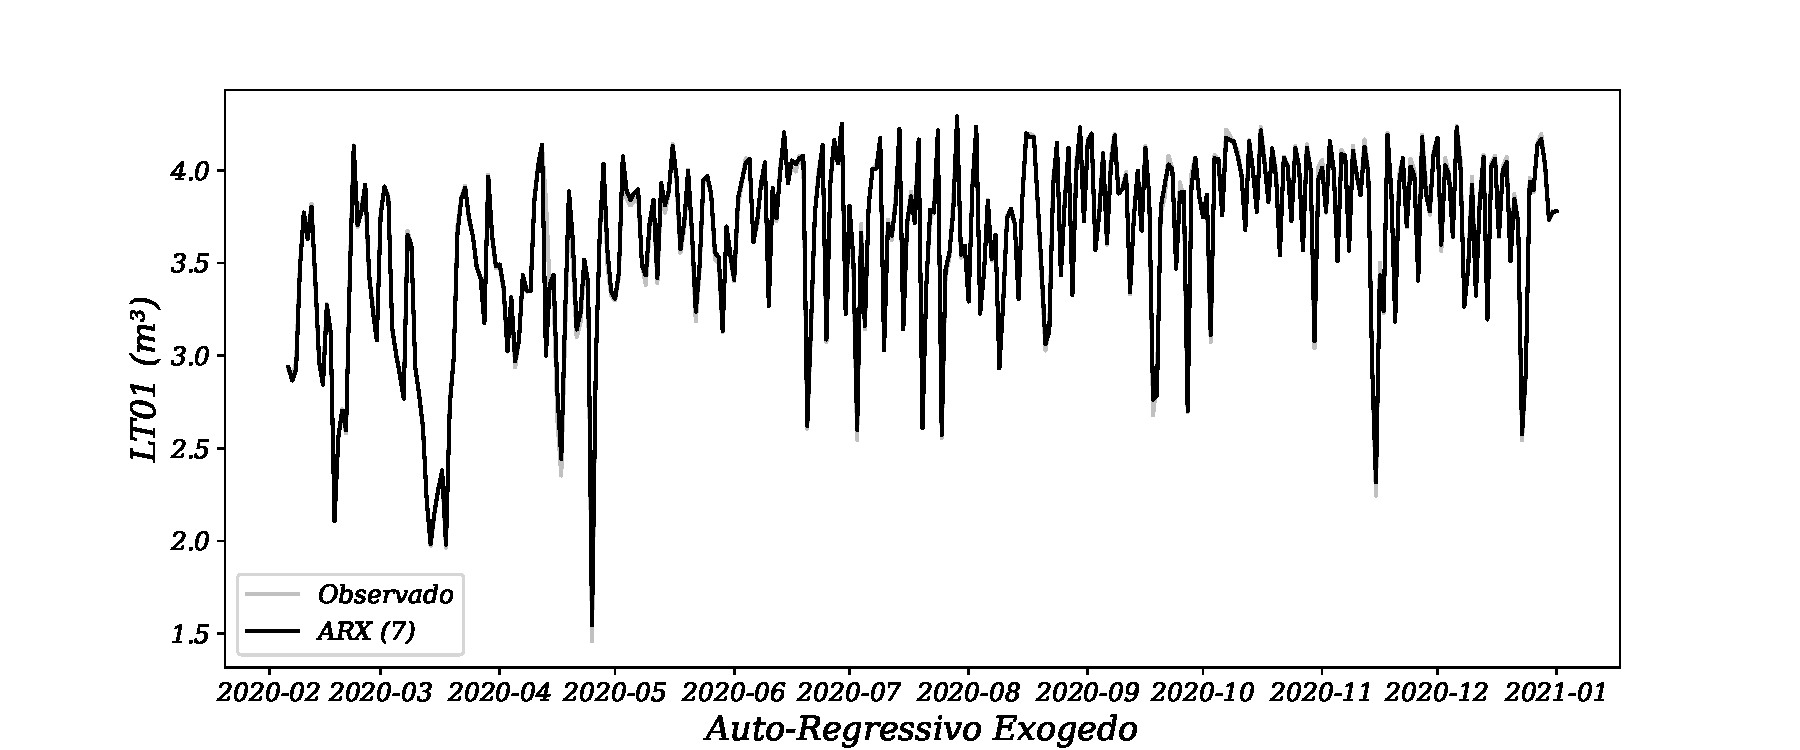
\includegraphics[width=\linewidth]{Modelos/Figuras/ARX}
			\caption{ARX (7)}
			\label{fig:1-arx}	
		\end{subfigure}
	
	\fonte{Elaboração própria a partir de dados da SANEPAR (2018 a 2020)}
\end{figure}




\begin{figure}[H]
	\centering
	\caption{Modelo MA(7) }
	\label{fig:1-ma}
	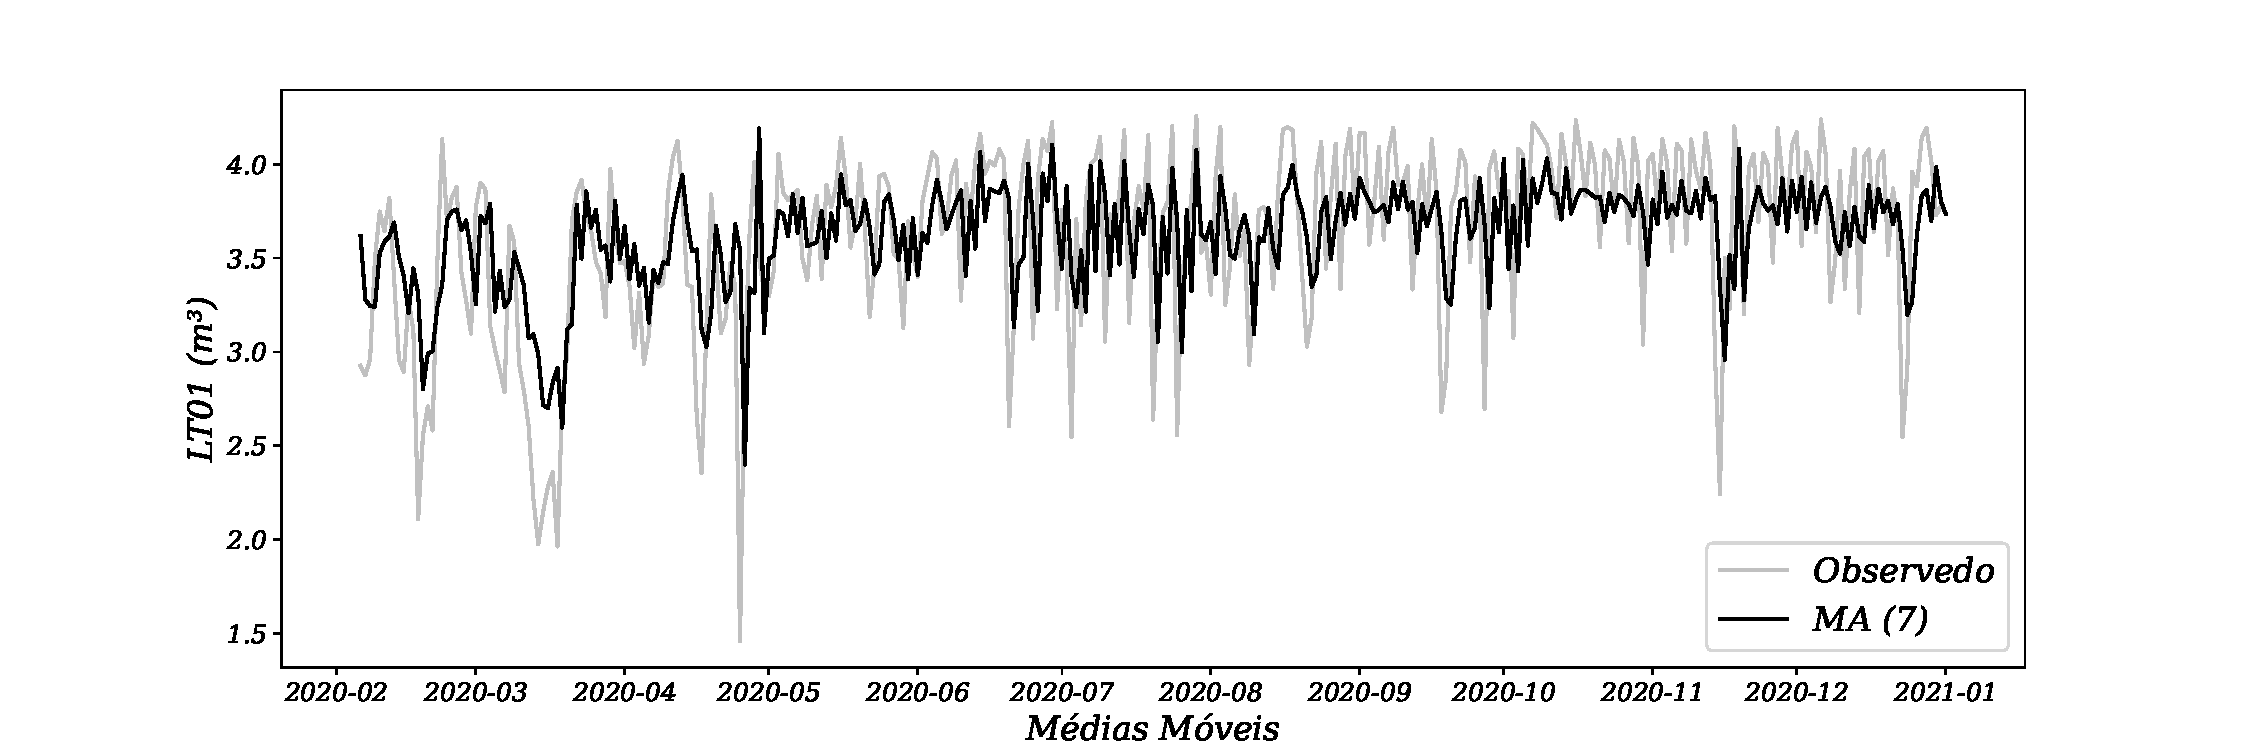
\includegraphics[width=1\linewidth]{Modelos/Figuras/MA}
	
	\fonte{Elaboração própria a partir de dados da SANEPAR (2018 a 2020)}
\end{figure}





\begin{figure}[H]
	\centering
	\caption{ARMA (7,7)}
	\label{fig:1-arma}
	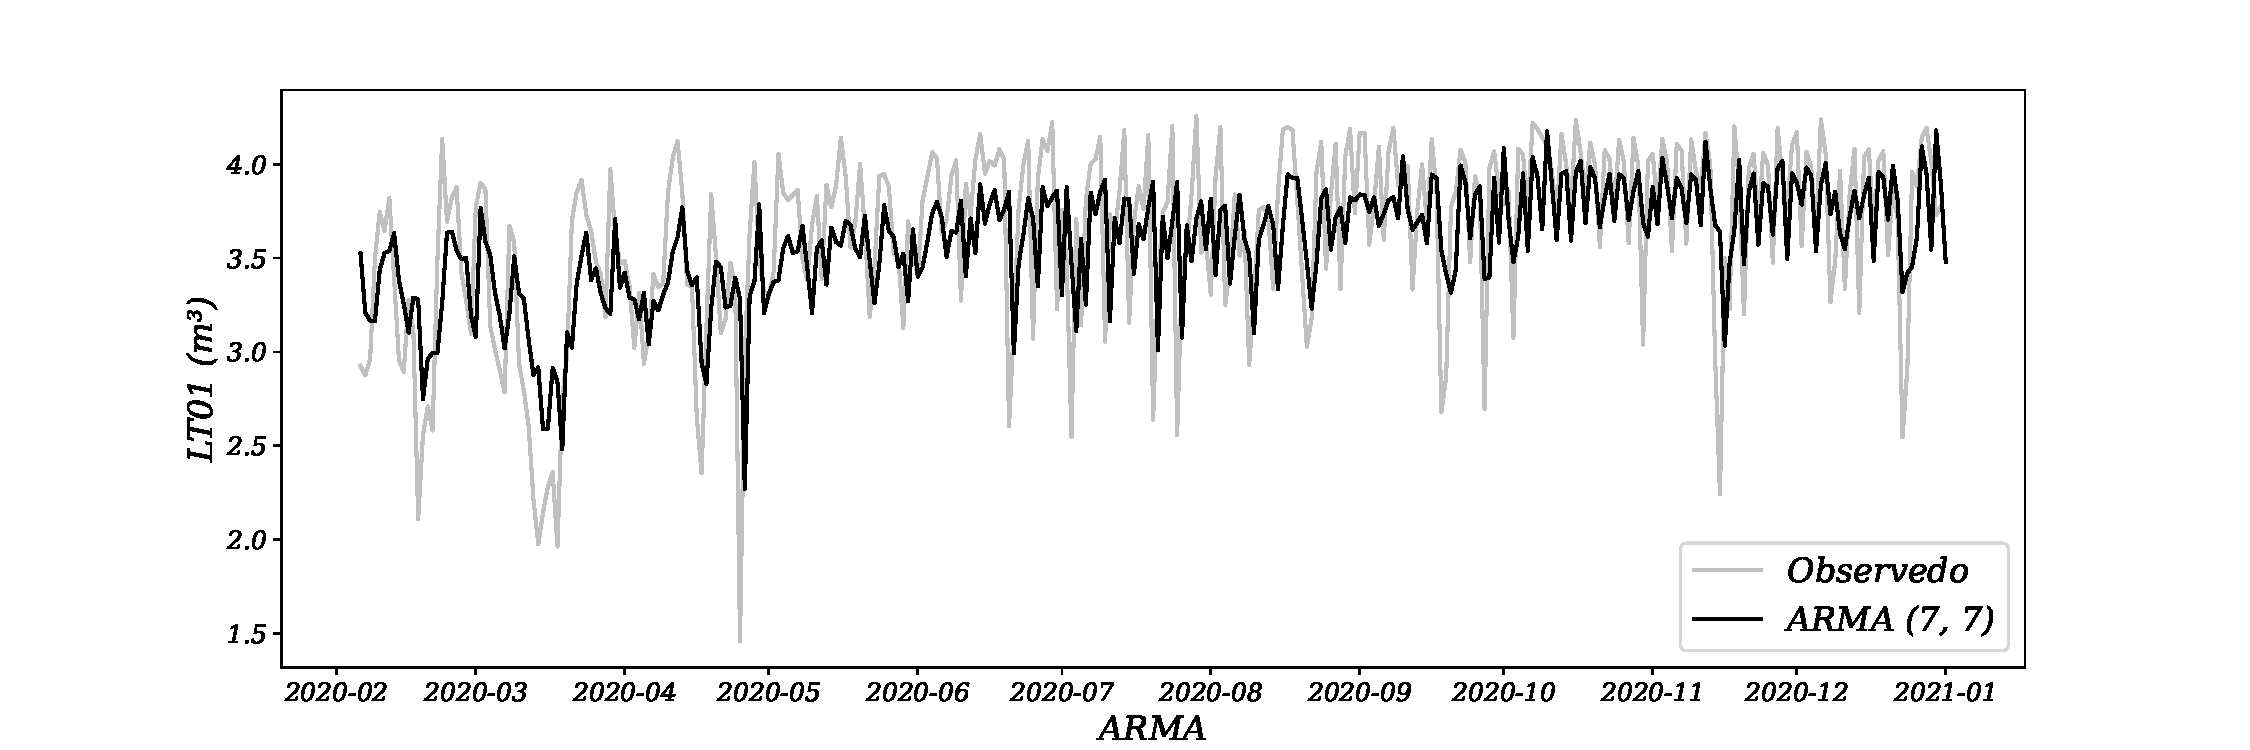
\includegraphics[width=1\linewidth]{Modelos/Figuras/ARMA}
	
	\fonte{Elaboração própria a partir de dados da SANEPAR (2018 a 2020)}
\end{figure}



\begin{figure}[H]
	\centering
	\caption{ARIMA (7,1,7)}
	\label{fig:1-arima}
	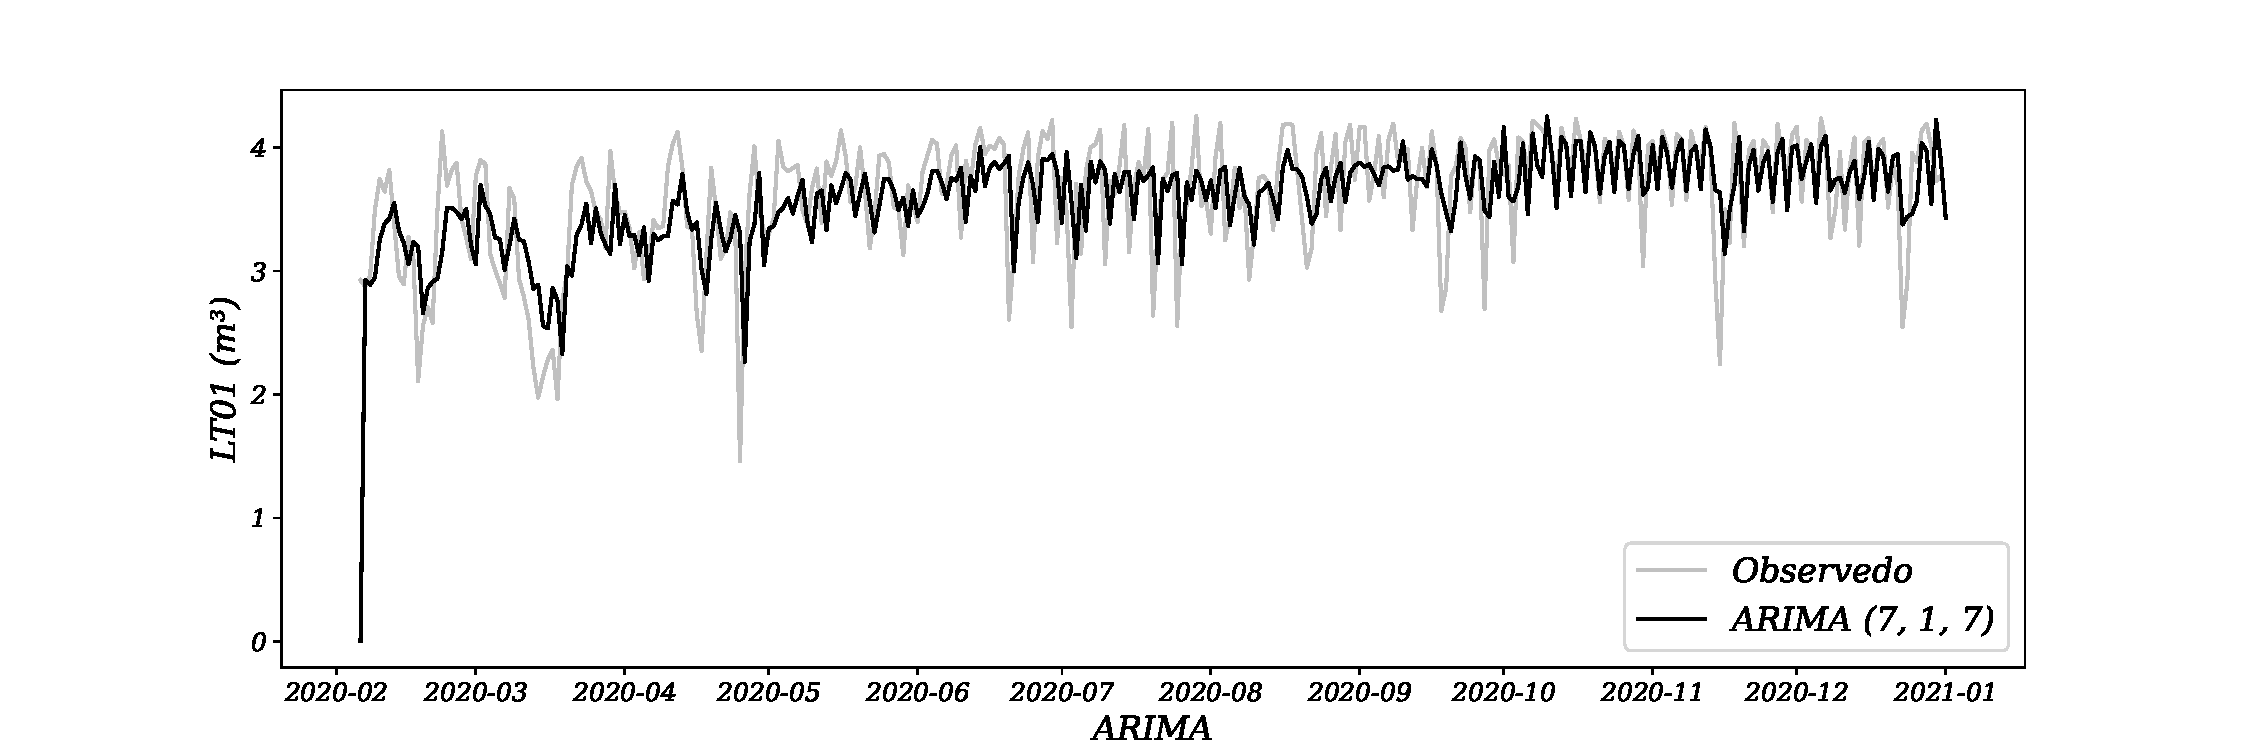
\includegraphics[width=1\linewidth]{Modelos/Figuras/ARIMA}
	
	Fonte: Elaboração própria a partir de dados da SANEPAR (2018 a 2020)
\end{figure}




\begin{figure}[H]
	\centering
	\caption{SARIMA $(7,1,7) (2,1,1)_{12}$}
	\label{fig:1-sarima}
	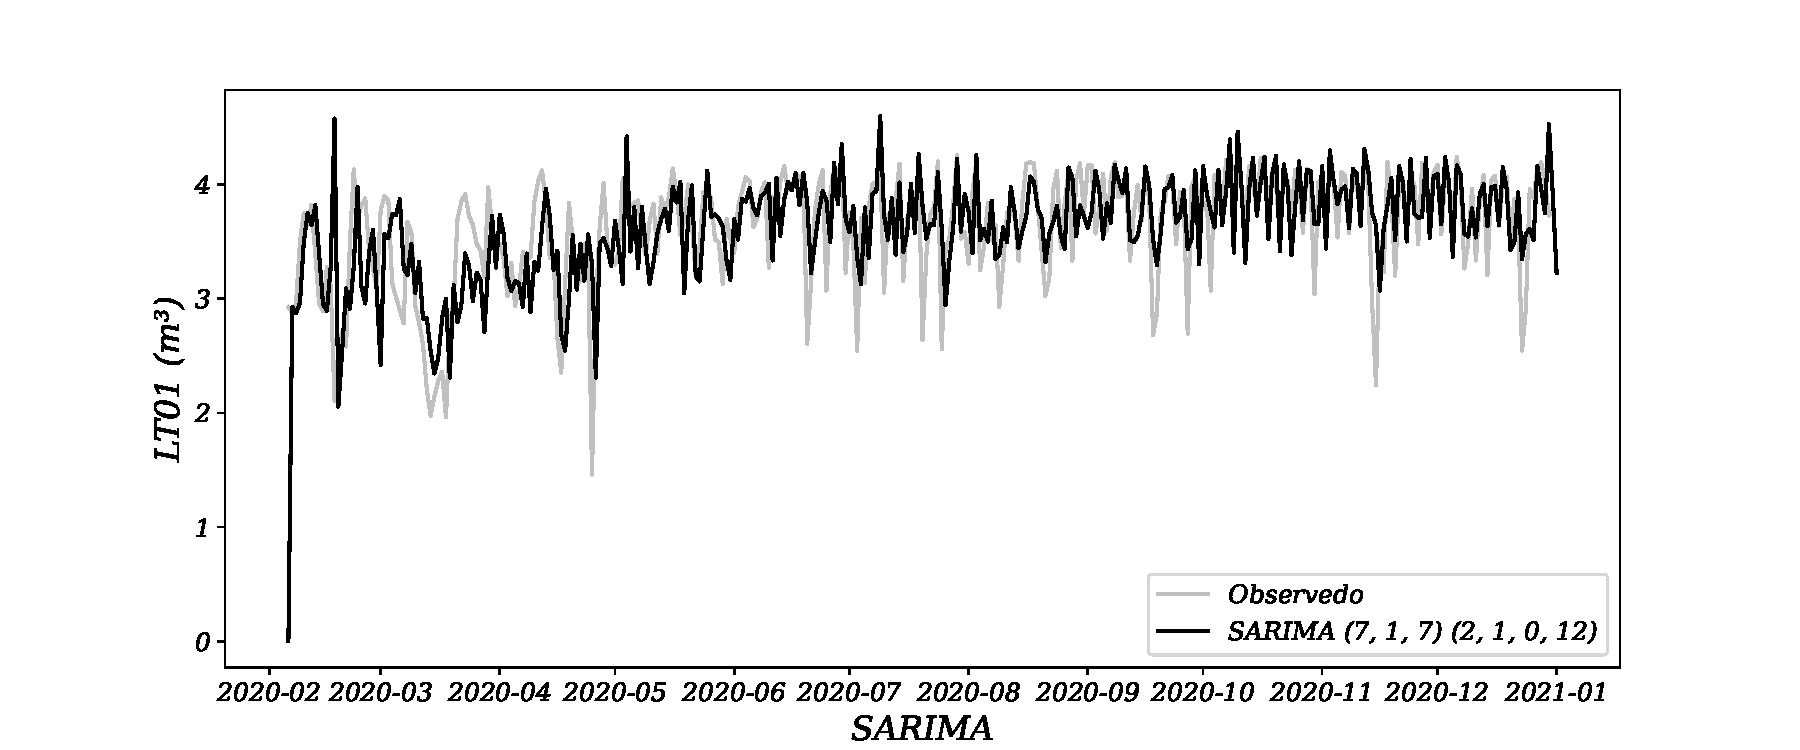
\includegraphics[width=1\linewidth]{Modelos/Figuras/SARIMA}
	
	\fonte{Elaboração própria a partir de dados da SANEPAR (2018 a 2020)}
\end{figure}



\begin{figure}[H]
	\centering
	\caption{Comparação entre ARIMAX e SARIMAX}
	\begin{subfigure}{1\textwidth}
			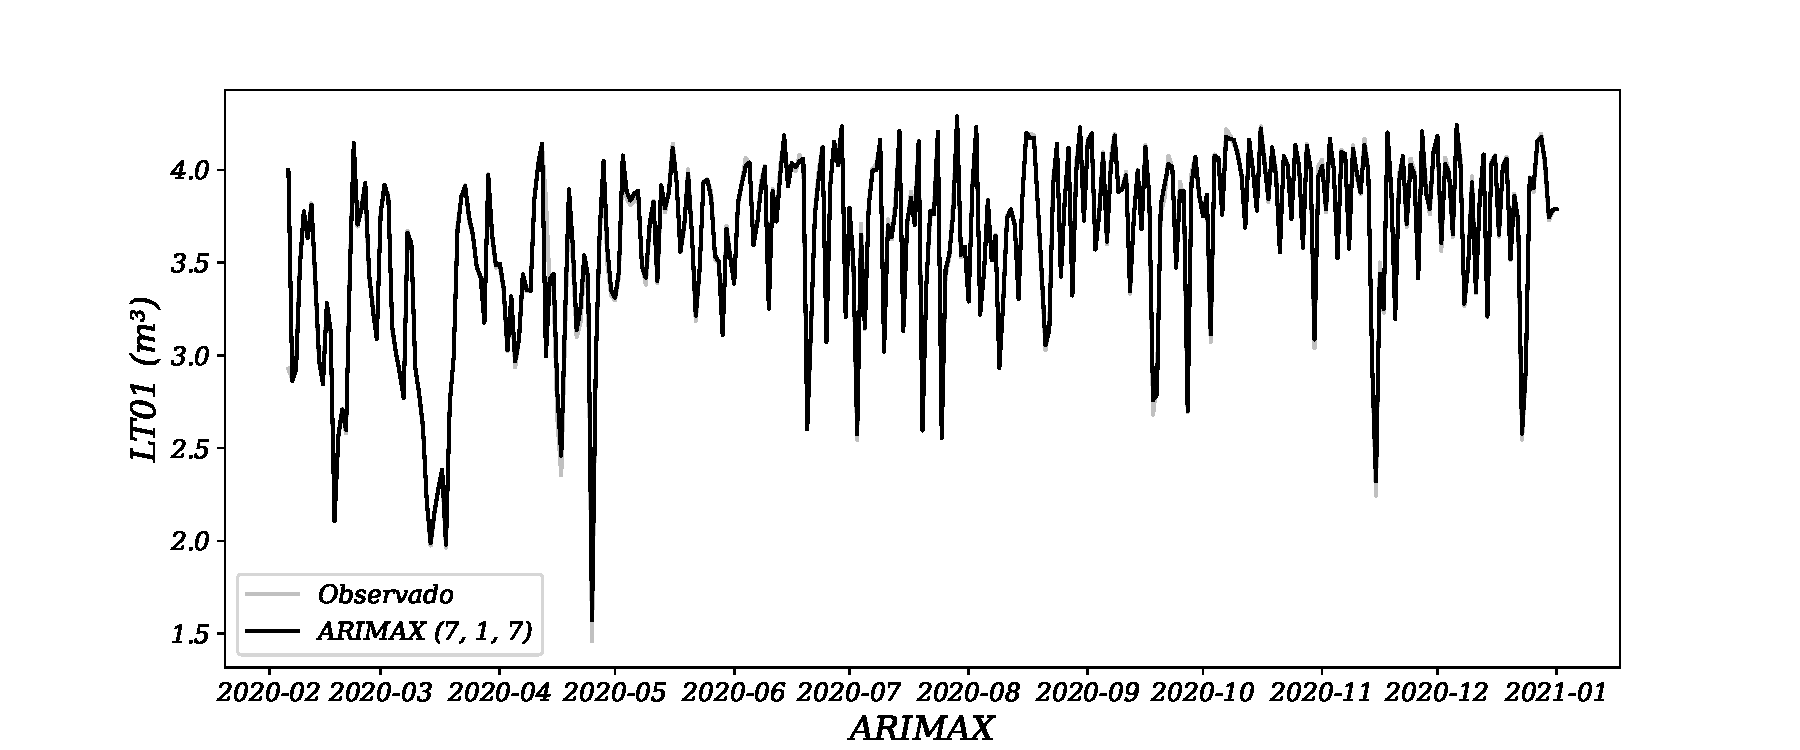
\includegraphics[width=\linewidth]{Modelos/Figuras/ARIMAX}
			\caption{ARIMAX $(7,1,7)$}
			\label{fig:1-arimax}
		\end{subfigure}
	\hfill
	
	\begin{subfigure}{1\textwidth}
			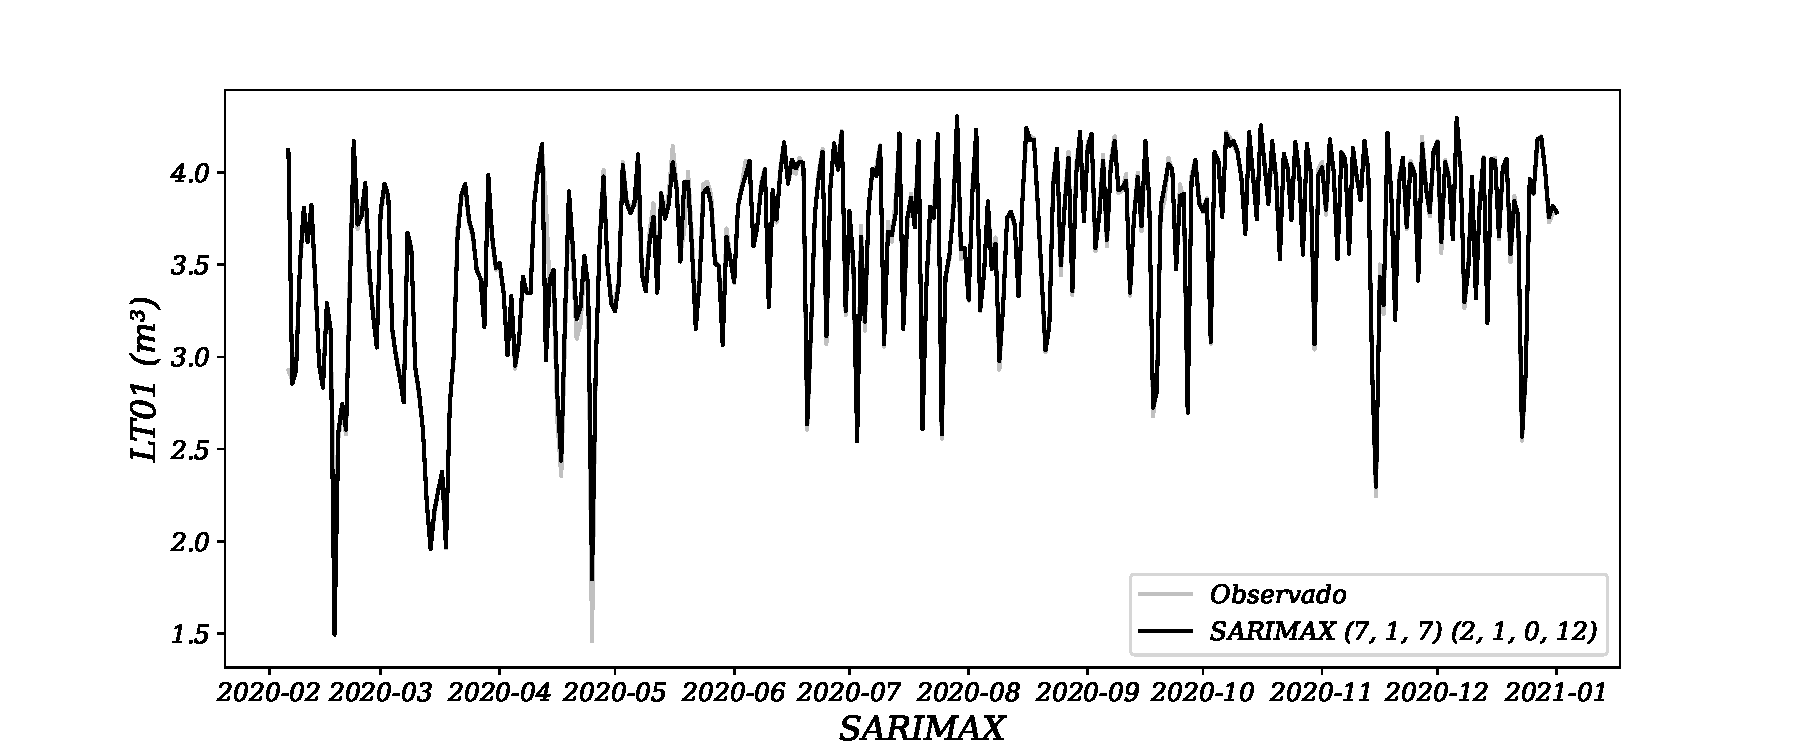
\includegraphics[width=\linewidth]{Modelos/Figuras/SARIMAX}
			\caption{SARIMAX $(7,1,7) (2,1,1)_{12}$}
			\label{fig:1-sarimax}	
		\end{subfigure}

		
	\fonte{Elaboração própria a partir de dados da SANEPAR (2018 a 2020)}
\end{figure}






\begin{figure}[H]
	\centering
	\caption{Previsões do modelo Prophet para o Reservatório LT01}\label{fig:prophet1}
	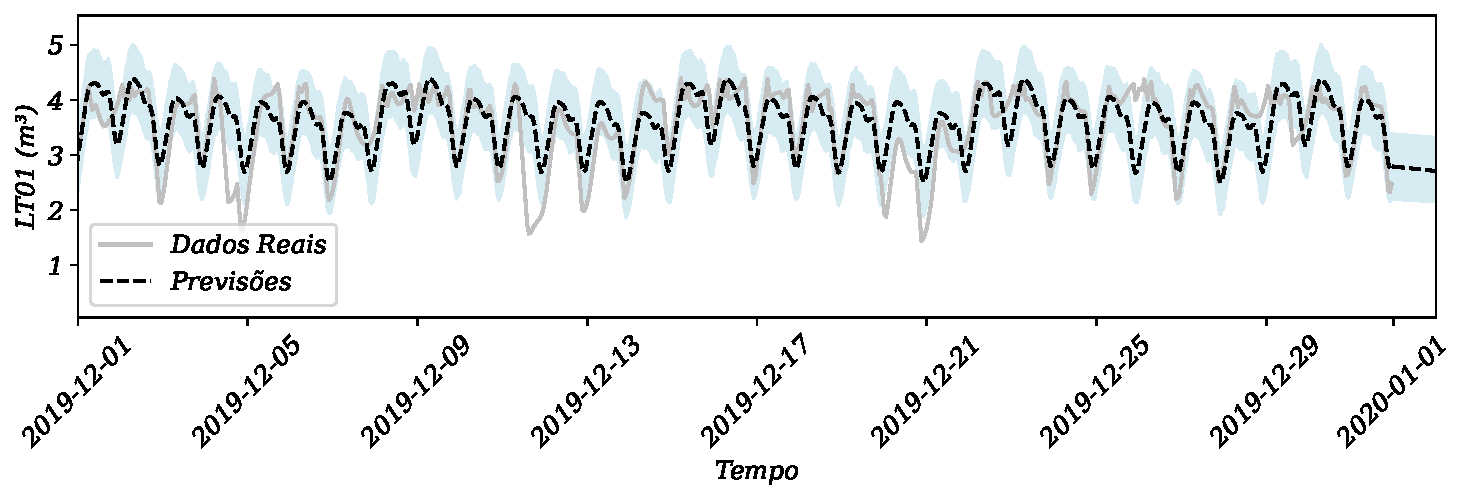
\includegraphics[width=1\linewidth]{Apendices/Figuras/modelagem-24h/prophet1}
	
	\fonte{Elaboração própria a partir de dados da SANEPAR (2018 a 2020)}
\end{figure}



\begin{figure}[H]
	\centering
	\caption{Regressão linear LT01 vs PT01 correlação 98\%}
	\label{fig:lr-lt01-m3}
	\includegraphics[width=0.82\linewidth]{"Modelos/Figuras/LR LT01 (m³)"}
	
	\fonte{Elaboração própria a partir de dados da SANEPAR (2018 a 2020)}
\end{figure}





\begin{figure}[H]
	\centering
	\caption{Regressão linear (LR) um passo a frente}
	\label{fig:1-regressao-linear}
	\includegraphics[width=1\linewidth]{Modelos/Figuras/regressão-linear}
	
	\fonte{Elaboração própria a partir de dados da SANEPAR (2018 a 2020)}
\end{figure}




\begin{figure}[H]
	\centering
	\caption{Regressor de \'Arvore de Decis\~ao }\label{fig:decision-tree-regressor}
	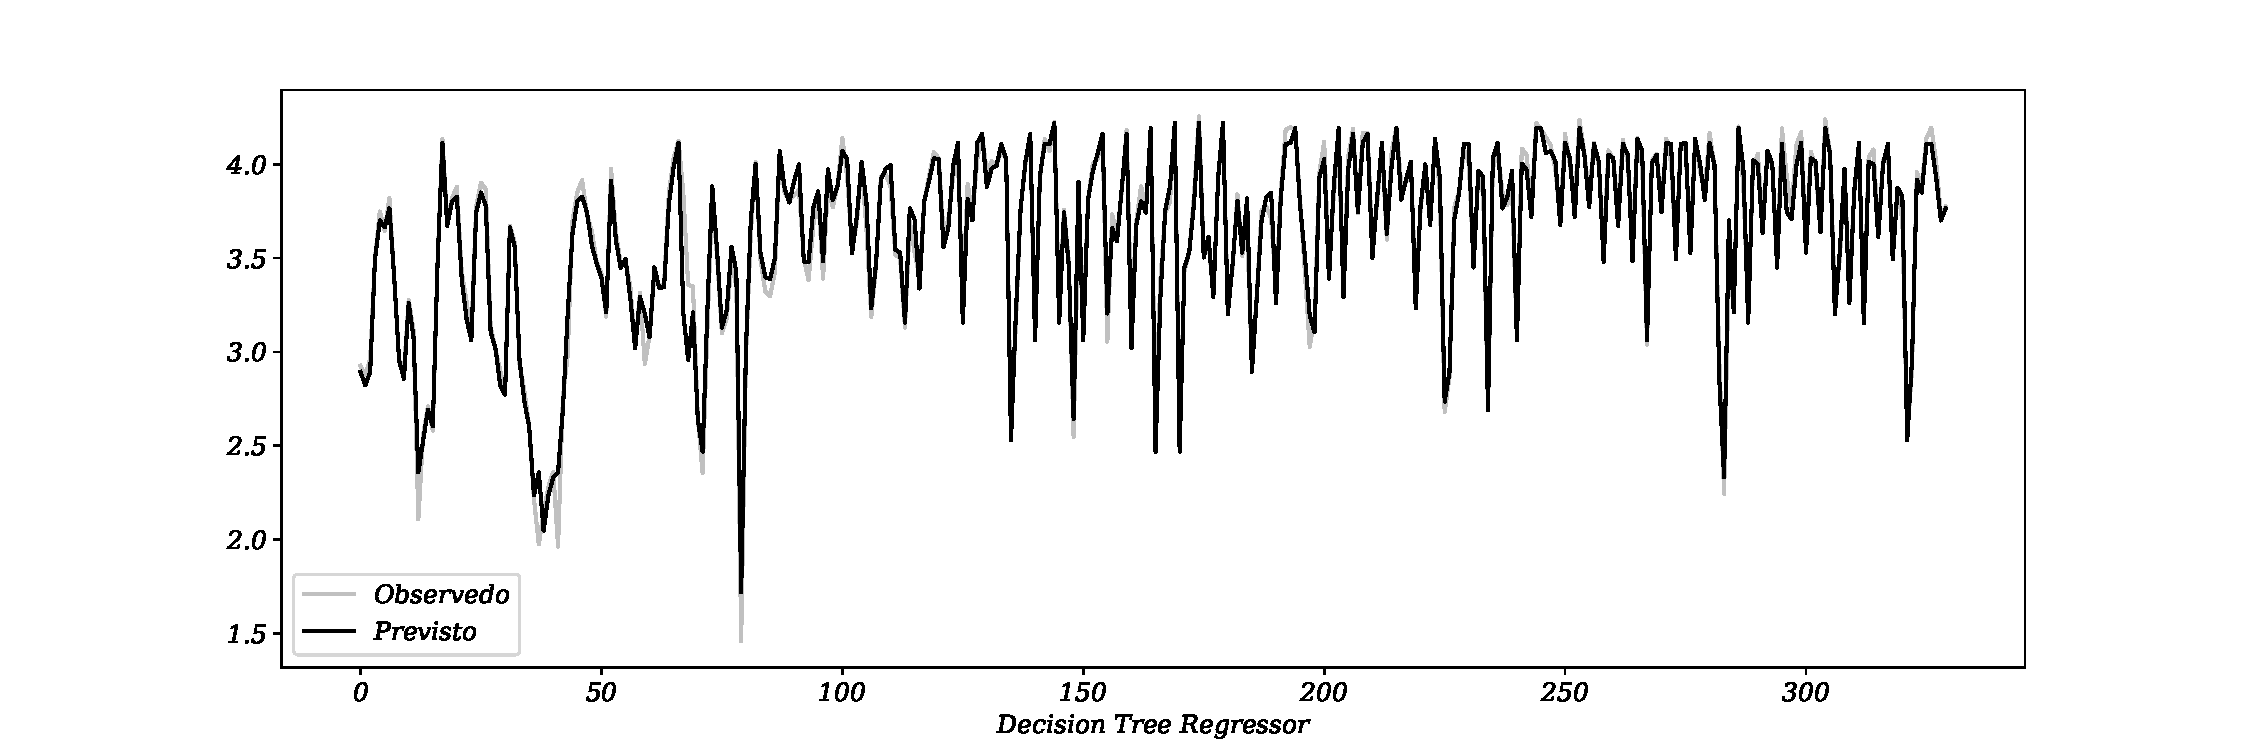
\includegraphics[width=1\linewidth]{Apendices/Figuras/modelagem-24h/Decision-Tree-Regressor}
	
	\fonte{Elaboração própria a partir de dados da SANEPAR (2018 a 2020)}
\end{figure}



\begin{figure}[H]
	\centering
	\caption{Regressão da Floresta Aleatória (RFR)}
	\label{fig:1-regressao-rfa}
	\includegraphics[width=1\linewidth]{Modelos/Figuras/regressão-rfa}
	
	\fonte{Elaboração própria a partir de dados da SANEPAR (2018 a 2020)}
\end{figure}





\begin{figure}[H]
	\centering
	\caption{A performance da regressão utilizando XGBoost e LightGBM é comparada}
	\label{fig:1-xgb-regressao}
	
	\begin{subfigure}{1\textwidth}
			\includegraphics[width=\linewidth]{Modelos/Figuras/xgb-regressão}
			\caption{Regressão XGBoost}	\label{fig:xgb}
		\end{subfigure}\hfill
	\begin{subfigure}{1\textwidth}
			\includegraphics[width=\linewidth]{Modelos/Figuras/lgbm-regressão}
			\caption{Regressão LightGBM}\label{fig:lgb}	
		\end{subfigure}
	
	\fonte{Elaboração própria a partir de dados da SANEPAR (2018 a 2020)}

\end{figure}	





